\documentclass{beamer}
%
% Choose how your presentation looks.
%
% For more themes, color themes and font themes, see:
% http://deic.uab.es/~iblanes/beamer_gallery/index_by_theme.html
%
\mode<presentation>
{
  \usetheme{Madrid}      % or try Darmstadt, Madrid, Warsaw, ...
  \usecolortheme{beaver} % or try albatross, beaver, crane  , ...
  \usefonttheme{default}  % or try serif, structurebold, ...
  \setbeamertemplate{navigation symbols}{}
  \setbeamertemplate{caption}[numbered]
} 

\usepackage[english]{babel}
\usepackage[utf8x]{inputenc}

\title[Data recovery of IoT]    {Probabilistic Recovery of Incomplete Sensed Data in IoT}
\author{Wang Liwei}
\institute{Auckland University}
\date{\today}

\begin{document}

\begin{frame}
  \titlepage
\end{frame}


\begin{frame} {From IoT to cognitive IoT}
   \
   {\Large What is cognitive IoT?\par}
  
  \vskip 1cm
      cognitive IoT is the use of cognitive computing technologies in combination with data generated by connected devices and the actions those devices can perform. 
\end{frame}

\begin{frame} {From IoT to cognitive IoT}
   \
   {\Large Cognition involves three key elements: \par}
  
  \vskip 1cm
  \begin{itemize}
      \item Understanding
      \item Reasoning
      \item Learning
  \end{itemize}
\end{frame}

\begin{frame} {From IoT to cognitive IoT}
   \
   {\Large Understanding\par}
  
  \vskip 1cm
      Being able to take in large volumes of both structured and unstructured data and derive meaning from it—that is, establish a model of concepts, entities and relationships. 
\end{frame}

\begin{frame} {From IoT to cognitive IoT}
   \
   {\Large Reasoning\par}
  
  \vskip 1cm
      Using that model to be able to derive answers or solve related problems without having the answers and solutions specifically programmed. 
\end{frame}

\begin{frame} {From IoT to cognitive IoT}
   \
   {\Large Learning\par}
  
  \vskip 1cm
      Being able to automatically infer new knowledge from data, which is a key component in understanding at scale. 
\end{frame}


\begin{frame} {From IoT to cognitive IoT}
   \
   {\Large Things to Think\par}
  
  \vskip 1cm
  \begin{itemize}
      \item Rate and scale of data generation:
      \item Computing’s movement into the physical world:
      \item Integration of multiple data sources and types: 
  \end{itemize}
    \vskip 3cm
    
   {\tiny IBM The Big Data  Analytics Hub\par}  
%{\tiny \texttt{Ref:https://www.ibmbigdatahub.com/blog/what-cognitive-iot?cm_mc_uid=47680 109391015373332594&cm_mc_sid_50200000=40739711538538014337} \par} 
\end{frame}




% Uncomment these lines for an automatically generated outline.
%\begin{frame}{Outline}
%  \tableofcontents
%\end{frame}

%\section{On the left Top}  


\begin{frame}{From IoT to cognitive IoT}
\begin{figure}
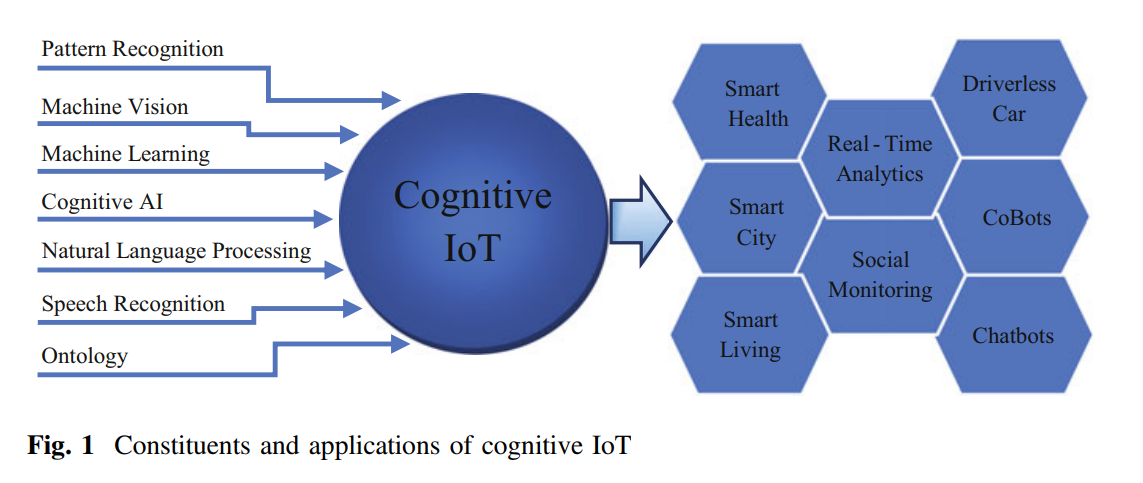
\includegraphics[width=1\textwidth]{CIOT1_application.png}
\caption{\label{fig:1} CIoT}
\end{figure}  
\end{frame}

\begin{frame} {From IoT to cognitive IoT}
   \
   {\Large Challenges of Cognitive IoT\par}
  
  \vskip 1cm
  \begin{itemize}
      \item Limited battery
      \item Diverse data types
      \item Privacy and security
      \item Training
      \item Device organization and data flow management
      \item Network and communication challenges
      \item Software and algorithms
      \item Societal apprehensions and ethics
      
  \end{itemize}
    \vskip 0.5cm
     
   {\tiny Sangaiah, Arun Kumar, Arunkumar Thangavelu, and Venkatesan Meenakshi Sundaram. "Cognitive Computing for Big Data Systems Over IoT." Gewerbestrasse 11 (2018): 6330.\par} 


\end{frame}  

\begin{frame}{Data Recovry(Matrix Missing element recovery)}
\begin{itemize}
  \item Your introduction goes here!
  \item Use \texttt{itemize} to organize your main points.
  \item what is  
  \item key
  \item what is 
  \item what is 
  \item what is 
  \item what is 
  \item what is 

  
\end{itemize}

\vskip 1cm

% \begin{block}{Examples}
% Wangliwei@gmail.com.
% \end{block}

\end{frame}

\section{Some \LaTeX{} Examples}

\subsection{Tables and Figures}

\begin{frame}{Tables and Figures}

\begin{itemize}
\item Use \texttt{tabular} for basic tables --- see Table~\ref{tab:widgets}, for example.
\item You can upload a figure (JPEG, PNG or PDF) using the files menu. 
\item To include it in your document, use the \texttt{includegraphics} command (see the comment below in the source  code).
\end{itemize}

% Commands to include a figure:


\begin{table}  
\centering
\begin{tabular}{l|r}
Item & Quantity \\\hline
Widgets & 42 \\
Gadgets & 13 \\
aaaa    &  0  \\
bbbb    &  0   \\
ccc     &  what
\end{tabular}
\caption{\label{tab:widgets}An example table.}
\end{table}

\end{frame}

\subsection{Mathematics}

\begin{frame}{Readable Mathematics}

Let $X_1, X_2, \ldots, X_n$ be a sequence of independent and identically distributed random variables with $\text{E}[X_i] = \mu$ and $\text{Var}[X_i] = \sigma^2 < \infty$, and let
$$S_n = \frac{X_1  + X_2 + \cdots + X_n}{n}
      = \frac{1}{n}\sum_{i}^{n} X_i$$
denote their mean. Then as $n$ approaches infinity, the random variables $\sqrt{n}(S_n - \mu)$ converge in distribution to a normal $\mathcal{N}(0, \sigma^2)$.

\end{frame}


% \begin{frame}{Show Pic}
% \begin{figure}
% \includegraphics[width=5cm]{WLW_3901.jpg}
% \caption{\label{fig:1}we are SSMIEL}
% \end{figure}  
% \end{frame}

\begin{frame}{Frame Title}
    
\end{frame}

\begin{frame}{Frame Title}
Thank you
\begin{enumerate}[Step 1:]
    \item test1
    \item test2
    \item test3

\end{enumerate}

    
\end{frame}

\end{document}
